\paragraph{Schedule Variance}\mbox{}\\[0,3cm]
\begin{table}[H]
    \centering
    \begin{tabular}{cccc}
        \rowcolor{greySWEight}
        \textcolor{white}{\textbf{Attività}} & 
        \textcolor{white}{\textbf{Abbreviazione}} &
        \textcolor{white}{\textbf{Valore Indice}}&
        \textcolor{white}{\textbf{Riscontro}}\\
		\textbf{Stesura Analisi dei Requisiti} & ADR & 1 & \textcolor{YellowOrange}{Accettabile}\\
		\textbf{Stesura Glossario} & GLO & -1 & \textcolor{ForestGreen}{Ottimale} \\
		\textbf{Stesura Piano di Progetto} & PDQ & 0 & \textcolor{ForestGreen}{Ottimale} \\
		\textbf{Stesura Piano di Qualifica} & PDP & -1 & \textcolor{ForestGreen}{Ottimale} \\
		\textbf{Stesura Norme di Progetto} & NDP & 1 & \textcolor{YellowOrange}{Accettabile} \\
		\textbf{Stesura Studio di Fattibilità} & SDF & 1 & \textcolor{YellowOrange}{Accettabile} \\

    \end{tabular}
    \caption{Schedule Variance nel periodo di Analisi}
\end{table}
\begin{figure}[H]
    \centering
	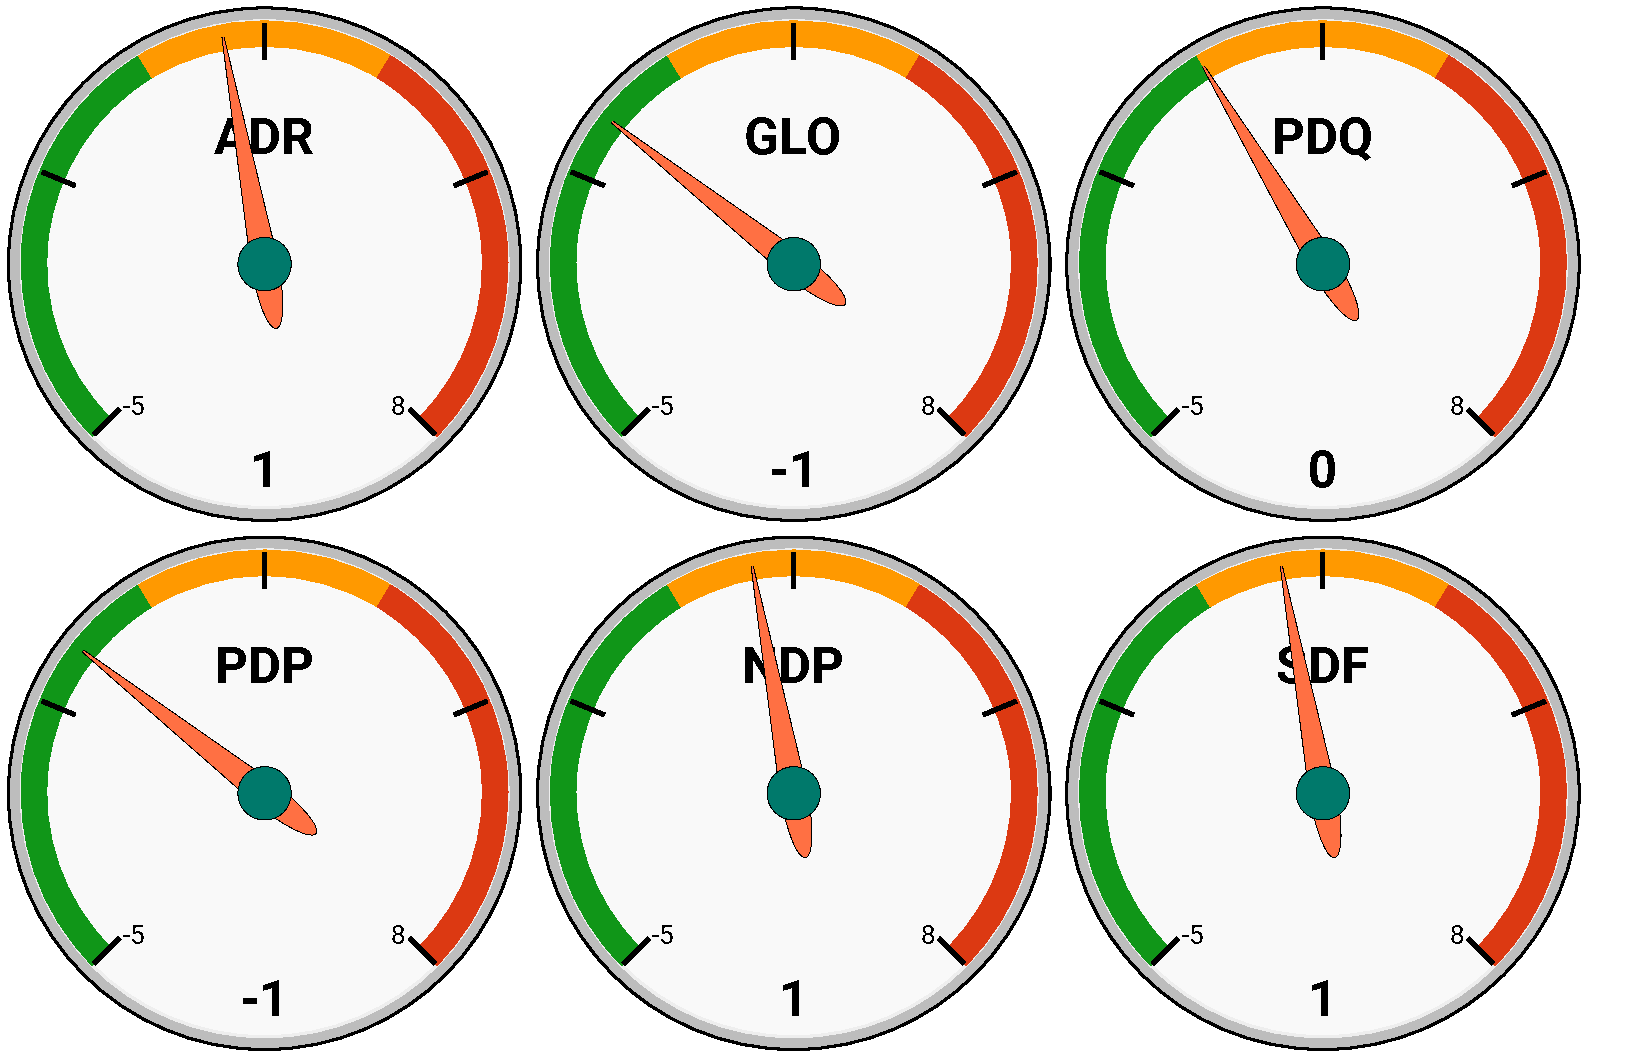
\includegraphics[width=1\linewidth]{sez/App_Esito/graph/AN_SV.pdf}
	\caption{Schedule Variance nel periodo di Analisi}
\end{figure}

\paragraph{Budget Variance}\mbox{}\\[0,3cm]
\begin{table}[H]
    \centering
    \begin{tabular}{cccc}
        \rowcolor{greySWEight}
        \textcolor{white}{\textbf{Abbreviazione}} &
        \textcolor{white}{\textbf{Valore Indice}}&
        \textcolor{white}{\textbf{Valore in €}}&
        \textcolor{white}{\textbf{Riscontro}}\\
        BV & 5,71\% & 200 & \textcolor{YellowOrange}{Accettabile}\\
    \end{tabular}
    \caption{Budget Variance nel periodo di Analisi}
\end{table}
\begin{figure}[H]
    \centering
	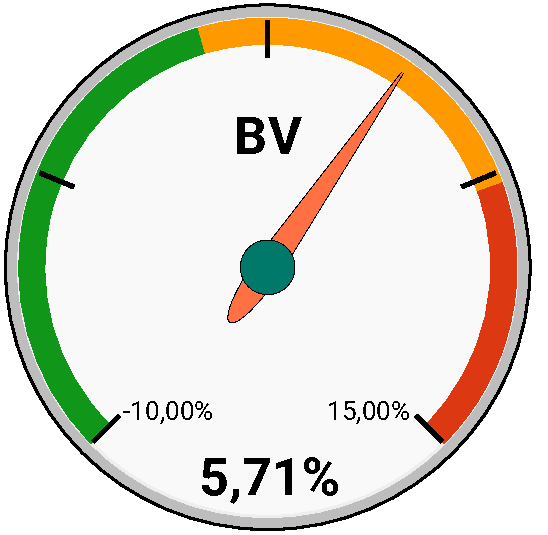
\includegraphics[height=4cm]{sez/App_Esito/graph/AN_BV.pdf}
	\caption{Budget Variance nel periodo di Analisi}
\end{figure}